\documentclass{l4dc2027}
% camera-ready: \documentclass[final]{l4dc2027}
\usepackage{iftex}
\ifXeTeX  % local builds use Tectonic (XeTeX); arXiv and Overleaf use pdfLaTeX, where the template's times package works
  \usepackage{fontspec}
  \setmainfont{texgyretermes}[Extension=.otf, UprightFont=*-regular, BoldFont=*-bold, ItalicFont=*-italic, BoldItalicFont=*-bolditalic]
\else
  \usepackage{times}
\fi
\usepackage{booktabs}
\usepackage{multirow}
\ifdefined\arxivpreprint  % set by scripts/package.sh for the arXiv source only
  \jmlrproceedings{}{Preprint}\jmlrvolume{}\jmlrpages{}\jmlryear{2026}
\fi
% AUTO-GENERATED by scripts/make_numbers.py from results/summary.json. Do not edit.
\newcommand{\ANsharp}{1\mbox{--}3}
\newcommand{\ARandThree}{0.57\mbox{--}0.67}
\newcommand{\ARandTwo}{0.41\mbox{--}0.51}
\newcommand{\ARemarkR}{0.84\mbox{--}0.96}
\newcommand{\ARemarkRone}{0.81\mbox{--}1.00}
\newcommand{\ARemarkSharp}{\ensuremath{-}119\mbox{--}\ensuremath{-}40}
\newcommand{\ARtheta}{0.19}
\newcommand{\ARthetaci}{[0.17, 0.21]}
\newcommand{\ATopThree}{0.88\mbox{--}0.90}
\newcommand{\ATopTwo}{0.78\mbox{--}0.82}
\newcommand{\AaccLast}{0.996}
\newcommand{\AaccZero}{0.94}
\newcommand{\AcCeilLin}{0.46}
\newcommand{\AcCeilMlp}{0.87}
\newcommand{\AcCtxDim}{6144}
\newcommand{\AcCtxMom}{0.50\mbox{--}0.53}
\newcommand{\AcCtxRpDim}{128}
\newcommand{\AcCtxRpMom}{0.08\mbox{--}0.09}
\newcommand{\AcCtxRpTheta}{0.01}
\newcommand{\AcCtxRpTrue}{0.01}
\newcommand{\AcCtxTheta}{0.33\mbox{--}0.37}
\newcommand{\AcCtxTrue}{0.32\mbox{--}0.36}
\newcommand{\AcFwDim}{4224}
\newcommand{\AcFwMom}{0.92}
\newcommand{\AcFwMomBone}{0.38}
\newcommand{\AcFwMomBtwo}{0.70\mbox{--}0.79}
\newcommand{\AcFwPcaDim}{128}
\newcommand{\AcFwPcaMom}{0.80\mbox{--}0.81}
\newcommand{\AcFwPcaTheta}{0.87}
\newcommand{\AcFwPcaTrue}{0.86}
\newcommand{\AcFwRpDim}{128}
\newcommand{\AcFwRpMom}{0.75\mbox{--}0.76}
\newcommand{\AcFwRpTheta}{0.84\mbox{--}0.86}
\newcommand{\AcFwRpTrue}{0.83\mbox{--}0.84}
\newcommand{\AcFwTheta}{0.90\mbox{--}0.91}
\newcommand{\AcFwThetaBone}{\ensuremath{-}0.01}
\newcommand{\AcFwThetaBtwo}{0.43\mbox{--}0.49}
\newcommand{\AcFwTrue}{0.89}
\newcommand{\AcLastMom}{0.29\mbox{--}0.31}
\newcommand{\AcLastTheta}{0.18\mbox{--}0.25}
\newcommand{\AcMeanMom}{0.68\mbox{--}0.71}
\newcommand{\AcMeanTheta}{0.58\mbox{--}0.61}
\newcommand{\AcQDim}{128}
\newcommand{\AcQMom}{0.28\mbox{--}0.29}
\newcommand{\AcQTheta}{0.18\mbox{--}0.25}
\newcommand{\AcQTrue}{0.18\mbox{--}0.25}
\newcommand{\AcResBestMom}{0.68\mbox{--}0.71}
\newcommand{\AcResBestTheta}{0.58\mbox{--}0.61}
\newcommand{\AcShuffled}{\ensuremath{-}0.01\mbox{--}0.01}
\newcommand{\AcfBayes}{0.86\mbox{--}0.94}
\newcommand{\AcfLin}{0.87\mbox{--}0.96}
\newcommand{\AcfSlope}{0.97\mbox{--}0.99}
\newcommand{\AdGD}{0.552}
\newcommand{\AdGDci}{[0.496, 0.616]}
\newcommand{\AdOLS}{0.271}
\newcommand{\AdOLSci}{[0.181, 0.379]}
\newcommand{\AdR}{0.005}
\newcommand{\AdRci}{[0.004, 0.006]}
\newcommand{\Aeta}{0.29}
\newcommand{\Afloor}{1.3}
\newcommand{\AfwR}{0.88\mbox{--}0.89}
\newcommand{\AfwRthree}{0.78\mbox{--}0.79}
\newcommand{\AjacBayes}{0.92}
\newcommand{\AjacOLS}{0.90}
\newcommand{\AjacTrue}{0.89}
\newcommand{\AkOnly}{0.44\mbox{--}0.48}
\newcommand{\AkvOne}{0.07\mbox{--}0.16}
\newcommand{\AkvThreeFour}{0.91\mbox{--}0.94}
\newcommand{\AkvTwoFour}{0.94\mbox{--}0.96}
\newcommand{\Alogtr}{0.66}
\newcommand{\AmlpTheta}{0.72}
\newcommand{\Amom}{0.30}
\newcommand{\Aprev}{0.27\mbox{--}0.90}
\newcommand{\Ar}{\ensuremath{-}0.007}
\newcommand{\Aratio}{1.59}
\newcommand{\AratioEnd}{2.04}
\newcommand{\Aratioci}{[1.56, 1.62]}
\newcommand{\AresidR}{0.08\mbox{--}0.14}
\newcommand{\Ashort}{1.23}
\newcommand{\Aslope}{\ensuremath{-}0.0000}
\newcommand{\AsteerYhat}{0.08}
\newcommand{\AtBayes}{0.057}
\newcommand{\AtTheory}{0.058}
\newcommand{\AtauCtxTwo}{0.91}
\newcommand{\AtauLastThree}{0.38\mbox{--}0.62}
\newcommand{\AtauYhat}{0.08}
\newcommand{\Ataurand}{0.067}
\newcommand{\Atausub}{0.0001}
\newcommand{\Atausubci}{[-0.0002, 0.0003]}
\newcommand{\AvOnly}{0.39\mbox{--}0.63}
\newcommand{\AyhatLfour}{0.97\mbox{--}0.98}
\newcommand{\AyhatLthree}{0.88\mbox{--}0.92}
\newcommand{\BKMLP}{0.019}
\newcommand{\BKNom}{0.075}
\newcommand{\BKOrc}{0.00026}
\newcommand{\BKOrcObs}{0.011}
\newcommand{\BKPer}{0.15}
\newcommand{\BKRLS}{0.019}
\newcommand{\BKSys}{0.011}
\newcommand{\BKSysNote}{worse than the transformer; with the true parameters and the same observation-only state it gets 0.011}
\newcommand{\BKTF}{0.0058}
\newcommand{\BKratio}{3.2}
\newcommand{\BPMLP}{0.0019}
\newcommand{\BPNom}{0.002}
\newcommand{\BPOrc}{8.9e-06}
\newcommand{\BPPer}{0.04}
\newcommand{\BPRLS}{5e-05}
\newcommand{\BPTF}{3.5e-05}
\newcommand{\BPratio}{58}
\newcommand{\BQMLP}{0.0021}
\newcommand{\BQNom}{0.0027}
\newcommand{\BQOrc}{4.5e-07}
\newcommand{\BQPer}{0.023}
\newcommand{\BQRLS}{0.037}
\newcommand{\BQTF}{0.0003}
\newcommand{\BfuncK}{0.42\mbox{--}0.43}
\newcommand{\BfuncP}{0.99}
\newcommand{\BfuncQ}{0.16\mbox{--}0.20}
\newcommand{\BfwKinvm}{0.64\mbox{--}0.68}
\newcommand{\BfwKmu}{0.68\mbox{--}0.72}
\newcommand{\BfwPg}{0.96}
\newcommand{\BfwPinvm}{0.97\mbox{--}0.98}
\newcommand{\BfwQinvm}{0.48}
\newcommand{\BfwQzeta}{0.98}
\newcommand{\BprobeKinvm}{0.34\mbox{--}0.35}
\newcommand{\BprobeKmu}{0.51\mbox{--}0.52}
\newcommand{\BprobePcoverm}{0.46\mbox{--}0.53}
\newcommand{\BprobePg}{0.82\mbox{--}0.86}
\newcommand{\BprobePinvm}{0.32\mbox{--}0.44}
\newcommand{\BprobeQg}{0.43\mbox{--}0.46}
\newcommand{\BprobeQinvm}{0.42\mbox{--}0.45}
\newcommand{\BprobeQzeta}{0.85\mbox{--}0.89}
\newcommand{\BresKinvm}{0.33\mbox{--}0.35}
\newcommand{\BresKmu}{0.51\mbox{--}0.52}
\newcommand{\BresPg}{0.82\mbox{--}0.86}
\newcommand{\BresPinvm}{0.32\mbox{--}0.44}
\newcommand{\BresQinvm}{0.42\mbox{--}0.45}
\newcommand{\BresQzeta}{0.88\mbox{--}0.89}
\newcommand{\BsteerK}{71}
\newcommand{\BsteerP}{42}
\newcommand{\BsteerQ}{39}
\newcommand{\CBCcvar}{390}
\newcommand{\CBCfail}{9.9}
\newcommand{\CBCinfo}{12.0}
\newcommand{\CBCmean}{22.69}
\newcommand{\CBCmed}{2.38}
\newcommand{\CBCpninety}{10.1}
\newcommand{\CCEDcvar}{11.7}
\newcommand{\CCEDfail}{1.4}
\newcommand{\CCEDinfo}{15.6}
\newcommand{\CCEDmean}{2.32}
\newcommand{\CCEDmed}{1.57}
\newcommand{\CCEDpninety}{3.7}
\newcommand{\CCEcvar}{8661.8}
\newcommand{\CCEfail}{30.2}
\newcommand{\CCEinfo}{10.0}
\newcommand{\CCEmean}{493.79}
\newcommand{\CCEmed}{2.81}
\newcommand{\CCEpninety}{407.3}
\newcommand{\CETCcvar}{16.7}
\newcommand{\CETCfail}{3.4}
\newcommand{\CETCinfo}{16.1}
\newcommand{\CETCmean}{2.95}
\newcommand{\CETCmed}{1.76}
\newcommand{\CETCpninety}{5.2}
\newcommand{\CFIXmean}{966}
\newcommand{\CFIXmed}{2.80}
\newcommand{\CORCinfo}{9.9}
\newcommand{\CTFcvar}{7612}
\newcommand{\CTFfail}{10.0}
\newcommand{\CTFfailRange}{9\mbox{--}11}
\newcommand{\CTFinfo}{14.2}
\newcommand{\CTFmean}{382.19}
\newcommand{\CTFmeanRange}{157\mbox{--}569}
\newcommand{\CTFmed}{1.69}
\newcommand{\CTFmedRange}{1.53\mbox{--}1.86}
\newcommand{\CTFpninety}{9.9}
\newcommand{\CTScvar}{11.4}
\newcommand{\CTSfail}{1.4}
\newcommand{\CTSinfo}{16.4}
\newcommand{\CTSmean}{2.58}
\newcommand{\CTSmed}{1.78}
\newcommand{\CTSpninety}{4.5}
\newcommand{\CbcMinusFt}{\ensuremath{-}359.50}
\newcommand{\CbcMinusFtci}{[-626.51, -130.78]}
\newcommand{\CfDNew}{0.028}
\newcommand{\CfDOls}{0.036}
\newcommand{\CfDTrain}{0.026}
\newcommand{\CfGap}{0.21\mbox{--}0.35}
\newcommand{\CfKv}{0.85\mbox{--}0.92}
\newcommand{\CfNsix}{9}
\newcommand{\CfRes}{0.52\mbox{--}0.71}
\newcommand{\CfSevenaN}{10}
\newcommand{\CfSevenaP}{<10^{-3}}
\newcommand{\CfSevenbN}{10}
\newcommand{\CfSevenbP}{<10^{-3}}
\newcommand{\CfSmallGap}{\ensuremath{-}0.07}
\newcommand{\CfSmallTauLate}{0.97}
\newcommand{\CfTauLate}{0.85\mbox{--}0.96}
\newcommand{\CfTauOne}{0.01\mbox{--}0.13}
\newcommand{\CfailStabBC}{2.8}
\newcommand{\CfailStabCED}{0.5}
\newcommand{\CfailStabETC}{2.0}
\newcommand{\CfailStabTF}{2.3}
\newcommand{\CfailStabTS}{0.9}
\newcommand{\CfailUnstBC}{25}
\newcommand{\CfailUnstCED}{3.3}
\newcommand{\CfailUnstETC}{6.3}
\newcommand{\CfailUnstTF}{27}
\newcommand{\CfailUnstTS}{2.6}
\newcommand{\Cflip}{0}
\newcommand{\CfracUnst}{31}
\newcommand{\CinfoCED}{\ensuremath{-}1.41}
\newcommand{\CinfoCEDci}{[-1.55, -1.29]}
\newcommand{\CinfoETC}{\ensuremath{-}1.91}
\newcommand{\CinfoETCci}{[-2.05, -1.79]}
\newcommand{\CinfoFtBc}{2.19}
\newcommand{\CinfoFtBcci}{[2.06, 2.37]}
\newcommand{\CinfoTS}{\ensuremath{-}2.18}
\newcommand{\CinfoTSci}{[-2.32, -2.05]}
\newcommand{\CmechBfwEarly}{0.69\mbox{--}0.81}
\newcommand{\CmechBfwEnd}{0.65\mbox{--}0.75}
\newcommand{\CmechBresEarly}{0.47\mbox{--}0.54}
\newcommand{\CmechBresEnd}{0.39\mbox{--}0.43}
\newcommand{\CmechCEErrEarly}{6.8}
\newcommand{\CmechCEErrEnd}{0.07}
\newcommand{\CmechGainEnd}{0.42\mbox{--}0.57}
\newcommand{\CmechGainErrEarly}{4.9}
\newcommand{\CmechGainErrEnd}{0.59}
\newcommand{\CmechGainMid}{0.21\mbox{--}0.37}
\newcommand{\CprobeB}{0.47}
\newcommand{\CprobeBhat}{0.47}
\newcommand{\CvsCED}{\ensuremath{-}379.87}
\newcommand{\CvsCEDci}{[-648.12, -152.71]}
\newcommand{\CvsCEDmed}{\ensuremath{-}0.10}
\newcommand{\CvsCEDmedci}{[-0.22, -0.00]}
\newcommand{\CvsETC}{\ensuremath{-}379.24}
\newcommand{\CvsETCci}{[-647.61, -152.08]}
\newcommand{\CvsETCmed}{0.01}
\newcommand{\CvsETCmedci}{[-0.09, 0.11]}
\newcommand{\CvsTS}{\ensuremath{-}379.61}
\newcommand{\CvsTSci}{[-647.87, -152.45]}
\newcommand{\CvsTSmed}{0.01}
\newcommand{\CvsTSmedci}{[-0.09, 0.11]}
\newcommand{\CwinsCED}{43}
\newcommand{\CwinsETC}{51}
\newcommand{\CwinsTS}{51}
\newcommand{\Hfivea}{583.52}
\newcommand{\Hfiveaci}{[146.79, 1179.44]}
\newcommand{\Hfiveb}{111.60}
\newcommand{\Hfivebci}{[-149.21, 343.32]}
\newcommand{\Hfived}{4.20}
\newcommand{\Hfivedci}{[4.06, 4.31]}
\newcommand{\HfourA}{0.0131}
\newcommand{\HfourAci}{[0.0128, 0.0134]}
\newcommand{\Hours}{15}
\newcommand{\PHfivea}{=0.015}
\newcommand{\PHfiveb}{=1.000}
\newcommand{\PHfived}{=0.001}
\newcommand{\PHfoura}{=0.001}
\newcommand{\PHfourc}{=1.000}
\newcommand{\PHfourd}{=1.000}
\newcommand{\PHonea}{=0.001}
\newcommand{\PHoneb}{=0.001}
\newcommand{\PHonec}{=1.000}
\newcommand{\PHthreea}{=1.000}
\newcommand{\PHthreeb}{=1.000}
\newcommand{\PHtwoa}{=1.000}
\newcommand{\PHtwob}{=0.001}
\newcommand{\RepFwMin}{0.90}
\newcommand{\RepFwMom}{0.92 $\pm$ 0.00}
\newcommand{\RepFwTheta}{0.91 $\pm$ 0.01}
\newcommand{\RepKv}{0.93 $\pm$ 0.01}
\newcommand{\RepKvMin}{0.91}
\newcommand{\RepN}{10}
\newcommand{\RepRatio}{1.58 $\pm$ 0.03}
\newcommand{\RepResCtx}{0.37 $\pm$ 0.07}
\newcommand{\RepResMax}{0.55}
\newcommand{\RepResQ}{0.24 $\pm$ 0.11}
\newcommand{\ScBaseRatio}{1.59}
\newcommand{\ScDeepJacEnd}{0.99}
\newcommand{\ScDeepRatio}{1.23}
\newcommand{\ScFourFinite}{0.282}
\newcommand{\ScFourJac}{0.72\mbox{--}0.73}
\newcommand{\ScFourJacEnd}{0.96\mbox{--}0.97}
\newcommand{\ScFourNP}{0.24}
\newcommand{\ScFourRatio}{4.4\mbox{--}4.9}
\newcommand{\ScFourTR}{0.276}
\newcommand{\ScLongJacEnd}{0.99}
\newcommand{\ScLongRatio}{1.22}
\newcommand{\ScLongRatioEnd}{1.38}
\newcommand{\ScMinBigJacEnd}{0.99}
\newcommand{\ScSmallJacEnd}{0.89}
\newcommand{\ScSmallRatio}{5.27}
\newcommand{\ScWideJacEnd}{0.99}
\newcommand{\ScWideRatio}{1.30}

\newcommand{\PENDING}[1]{\textbf{[#1 pending]}}

\title[In-context adaptation to unknown physics]{What a Transformer Learns When It Adapts to Unknown Physics\\ In-Context: Probing, Patching and Controlling}

\coltauthor{\Name{Anuar Zhambakin} \Email{https://github.com/nonberw/suss}\\
 \addr Independent researcher}

\begin{document}

\maketitle

\begin{abstract}%
Sequence models that adapt to unknown dynamics from their own history are widely used in robot learning, but
what they compute is unclear. We study this question in small transformers trained from scratch, in a
pre-registered design with exact optimal references and causal interventions, in three settings: linear systems
with unknown parameters, MuJoCo pendulum, sliding-block and bouncing-ball physics, and in-context adaptive control.
We prove an exact Bayes-risk identity for in-context prediction under any non-anticipating policy, which gives a
parameter-free context-length law. We also prove a closed-loop identity: the information gained along unexcited
directions equals the excitation energy. The trained predictors are Bayes-optimal while data are scarce, then
settle at an approximation floor. Our pre-registered mechanism, a linearly readable and causally used parameter
estimate in the residual stream, is rejected: the best probe reaches $R^2{=}\ARtheta$, and steering and patching along it
have no effect. Exploratory analyses locate the estimate instead in the attention key--value memory. Fast weights
decode it ($R^2{=}\AfwR$, against $\le\AresidR$ for the residual stream). The predictor's query Jacobian equals the Bayes
estimate ($R^2{=}\AjacBayes$). Patching \emph{only} context keys and values transfers $\AkvThreeFour$ of the behaviour. The same
holds for physical parameters in MuJoCo; on stick--slip friction the transformer beats physics-feature regression by $\BKratio\times$.
A transformer controller, trained by imitation and then on closed-loop cost, learns to excite the plant with no identification objective (\Hfived\ nats more information than exploration-free certainty equivalence) and matches classical adaptive controllers in median cost, but it fails on \CTFfail\% of plants, almost all open-loop unstable, against \CCEDfail\% for dithered certainty equivalence.
Code, pre-registration, deviation log and all numbers are public.

\end{abstract}

\begin{keywords}%
in-context learning, adaptive control, system identification, dual control, mechanistic interpretability
\end{keywords}

\section{Introduction}

A robot picking up an unfamiliar object, or a legged robot stepping onto ice, must adapt to physics it does not
know from a few seconds of interaction. A popular recipe trains a sequence model across randomised physics and lets it
adapt \emph{in context}, from its own history, with no gradient steps at deployment~\citep{kumar2021rma,duan2016rl2,forgione2023from,busetto2024one}.
These models work, but it is not clear what they compute. Do they identify the plant and then plan? Do they
implement a classical estimator? Do they explore?

For linear-Gaussian dynamics these questions have exact answers, so they can be tested. Transformers trained on
random linear systems are known to \emph{behave} like the Kalman filter or least
squares~\citep{balim2023can,akram2026transformers}. They are also known to be \emph{able to represent} such
estimators~\citep{goel2024can,cole2025incontext,vladarean2026learning}. What has not been measured is what is inside
a trained in-context system-identifier, or what an in-context \emph{controller} does about the dual effect. The second
question matters because, under exploration-free feedback, closed-loop data do not identify the plant~\citep{feldbaum1960dual,astrom1995adaptive,ljung1999system}.
\citet{akram2026transformers} list the first question as future work.

We study both questions in a pre-registered design. Hypotheses, metrics, seeds and tests were committed before the
main experiments, and deviations are logged. The design combines exact optimal references, causal interventions and
three settings of increasing difficulty: linear prediction, MuJoCo contact physics~\citep{todorov2012mujoco}, and adaptive control.
Our contributions:
\begin{itemize}
\item \textbf{Theory (\S\ref{sec:theory}).} An exact Bayes-risk identity for in-context prediction under any
non-anticipating policy, with a parameter-free context-length law $t\,\mathcal{R}^\star_t\to np\sigma^2$. A
closed-loop non-identifiability identity: the information gained along unexcited directions equals the excitation energy, and is
exactly zero under pure feedback. A two-layer construction that gathers the exact sufficient statistics, and a
first-order account of how a near-uniform attention head can apply a parameter estimate that is stored only in its
key--value memory (Remark~\ref{rem:fw}).
\item \textbf{What the trained predictor computes (\S\ref{sec:expa}).} It is Bayes-optimal while data are scarce, and
then it settles at an approximation floor. Our pre-registered mechanism, a linearly readable and causally used parameter estimate in the
residual stream, is \emph{rejected}: the probe reaches $R^2{=}\ARtheta$, and steering and subspace patching have no effect. Exploratory analyses show instead that the estimate lives
in the \emph{key--value memory} of the last two blocks. It is readable from the fast weights ($R^2{=}\AfwR$), it equals the predictor's
query Jacobian ($R^2{=}\AjacBayes$ against the Bayes estimate), and patching only context keys and values transfers
$\AkvThreeFour$ of the behaviour.
\item \textbf{Contact physics (\S\ref{sec:expb}).} On a pushed block with Coulomb friction the transformer beats
physics-feature RLS by $\BKratio\times$, and on a pendulum it beats RLS even though RLS has the true model class. Physical parameters follow the same pattern:
they are weakly readable from activations ($1/m$: $R^2{=}\BprobePinvm$), but strongly readable from the key--value memory ($\BfwPinvm$) and from the model's
input sensitivity ($r{=}\BfuncP$).
\item \textbf{In-context control (\S\ref{sec:expc}).} A transformer controller trained by imitation and then on cost discovers excitation (\Hfived\ nats of information above exploration-free certainty equivalence, of which \CinfoFtBc\ come from cost training), and it matches dithered certainty equivalence and Thompson sampling in median cost. Its failure rate, however, is \CTFfail\% against \CCEDfail\%, concentrated on open-loop-unstable plants, and cost fine-tuning makes those failures more severe. The controller stores its estimate of the actuation matrix in the same key--value memory.
\end{itemize}

\section{Related work}

\paragraph{In-context learning of function classes.} Transformers trained on random regression tasks match least
squares~\citep{garg2022what}. Behaviourally they interpolate between ridge and OLS, and probes recover intermediate
quantities in static regression~\citep{akyurek2022learning}. They can implement GD~\citep{vonoswald2023transformers,ahn2023transformers,zhang2023trained},
higher-order iterations~\citep{fu2023transformers} and algorithm selection~\citep{bai2023transformers}, and they
approximate posterior predictives~\citep{muller2022transformers,raventos2023pretraining}. We move these questions to
dynamical, closed-loop data, where the regressors depend on the past and on the policy. There the dual effect has no analogue in i.i.d.\ regression.

\paragraph{In-context learning of dynamical systems.} Meta-trained transformers predict and filter unseen linear and
nonlinear systems~\citep{forgione2023from,piga2023adaptation,busetto2023incontext,balim2023can,akram2026transformers}
and can serve as contextual controllers for a system class~\citep{busetto2024one}. Constructions and approximation
theory exist for Kalman filtering~\citep{goel2024can}, for least-squares learning of LDS with depth
separation~\citep{cole2025incontext}, and for single linear-attention layers~\citep{vladarean2026learning}. All of these are
either behavioural or representational. None of them intervenes on a trained model.

\paragraph{Adaptation from history and in-context RL.} RMA~\citep{kumar2021rma} regresses a history encoding onto
privileged physical parameters. Probing such latents gives mixed results~\citep{chamachot2026evaluating}, and decoding
them can need a learned generative model~\citep{zhang2026interpreting}. Meta-RL agents can learn to
explore~\citep{duan2016rl2,zintgraf2020varibad}; algorithm distillation imitates learning
histories~\citep{laskin2022incontext}; and in-context RL algorithms are provably representable in tabular
MDPs~\citep{liang2026transformers}. In adaptive LQR, certainty equivalence with dithering is
rate-optimal~\citep{mania2019certainty,simchowitz2020naive}. We use these methods as baselines and ask whether a
transformer controller, trained by imitation and then on cost, discovers the excitation they prescribe.

\paragraph{Interpretability tools and fast weights.} We use linear probes~\citep{alain2016understanding} and activation
patching~\citep{zhang2024towards,heimersheim2024how}. Our probes are always paired with interventions, and the probe
targets are \emph{estimator} quantities, which are distinct from the ground truth. The view of attention as reading and writing
\emph{fast weights}~\citep{ba2016using,schlag2021linear}, and its dual form as implicit gradient
descent~\citep{dai2023why,vonoswald2023transformers}, motivates our key--value analysis. To our knowledge, it has not
been used to localise a physical parameter estimate in a trained model.

\section{Theoretical background}\label{sec:theory}
The results of this section are standard (Bayesian ridge regression, closed-loop identifiability, and attention as
fast weights), restated for in-context predictors under closed-loop data. We include short proofs for completeness and
claim no novelty; their role is to turn the questions of \S\ref{sec:intro} into measurable gaps.

\paragraph{Setting.} A plant $x_{s+1}=\theta z_s+w_s$ with regressor $z_s=(x_s,u_s)\in\mathbb{R}^p$, unknown
$\theta=[A\;B]\in\mathbb{R}^{n\times p}$, and noise $w_s\sim\mathcal{N}(0,\sigma^2 I_n)$ i.i.d.\ and independent of
everything else. The rows $\theta_i$ of $\theta$ have independent priors $\mathcal{N}(0,\Lambda_0^{-1})$. Inputs are chosen by an
arbitrary \emph{non-anticipating} policy: $u_s$ is a measurable function of the past data
$\mathcal{D}_s=(x_0,u_0,\dots,x_s)$ and of independent randomness, so it does not depend on $\theta$ except through
$\mathcal{D}_s$. An \emph{in-context predictor} is any map $\hat y_t=f_t(\mathcal{D}_t,u_t)$, of which a causal transformer
is one example. Write $S_t=\sum_{s<t} z_s z_s^\top$ and $C_t=\sum_{s<t} z_s x_{s+1}^\top$.

\begin{theorem}[Bayes risk of in-context prediction; Bayesian ridge regression]\label{thm:bayes}
Under the untruncated Gaussian prior, for every in-context predictor and every $t$,
\begin{equation}
\mathbb{E}\,\|\hat y_t-\theta z_t\|^2\;\ge\;\mathcal{R}^\star_t:=n\sigma^2\,\mathbb{E}\big[z_t^\top(\sigma^2\Lambda_0+S_t)^{-1}z_t\big],
\label{eq:bayes}
\end{equation}
with equality iff $\hat y_t=C_t^\top(\sigma^2\Lambda_0+S_t)^{-1}z_t$ almost surely. This is ridge regression, i.e.\ RLS
initialised at the prior.
\end{theorem}
\begin{proof}[Proof sketch]
The policy factors of the likelihood do not depend on $\theta$, so each row of $\theta$ has a Gaussian posterior with precision $\Lambda_0+\sigma^{-2}S_t$; the bias--variance identity then gives \eqref{eq:bayes}. Appendix~\ref{app:proofs}.
\end{proof}

\begin{corollary}[A parameter-free context-length law]\label{cor:law}
Fix $\theta$ and suppose that, conditionally on $\theta$: (a)~$S_t/t\to\Sigma_\theta\succ0$ almost surely; (b)~$\mathbb{E}[z_tz_t^\top\mid\theta]\to\Sigma_\theta$;
(c)~the families $\{t\,z_t^\top(\sigma^2\Lambda_0+S_t)^{-1}z_t\}_t$ and $\{\|z_t\|^2\}_t$ are uniformly integrable. Then
the conditional Bayes risk satisfies $t\,\mathcal{R}^\star_t(\theta)\to n\,p\,\sigma^2$. If, in addition,
$\sup_t t\,\mathcal{R}^\star_t(\theta)$ is integrable over the prior, then $t\,\mathcal{R}^\star_t\to np\sigma^2$. The limit
does not depend on the prior, on $\theta$, or on the input distribution, because
$\operatorname{tr}(\Sigma_\theta^{-1}\Sigma_\theta)=p$ whatever $\Sigma_\theta$ is. Conditions (a)--(b) are standard
for stable plants driven by i.i.d.\ inputs (as in Experiment~A); we check the limit numerically rather than verify (c).
\end{corollary}
\begin{proof}[Proof sketch]
$t(\sigma^2\Lambda_0+S_t)^{-1}\to\Sigma_\theta^{-1}$ a.s.; uniform integrability exchanges limit and expectation; and $\operatorname{tr}(\Sigma_\theta^{-1}\Sigma_\theta)=p$. Full proof in Appendix~\ref{app:proofs}.
\end{proof}

Theorem~\ref{thm:bayes} turns ``is the transformer Bayes-optimal?'' into a measurable gap. Corollary~\ref{cor:law}
gives a target curve $\mathcal{R}^\star_t\approx np\sigma^2/t$ that involves no fitted constants. (In
Experiment~A, the prior is truncated to stable $A$. The exact optimum is then the truncated posterior mean, which
we compute by Monte Carlo. The truncation only matters at short contexts.)

\begin{proposition}[Closed-loop non-identifiability; the dual effect]\label{prop:ident}
Let the policy be $u_s=Kx_s+\varepsilon_s$ for a fixed $K\in\mathbb{R}^{m\times n}$ and an excitation sequence
$\varepsilon_s$. For any $b\in\mathbb{R}^m$, let $v_b=(-K^\top b,\;b)\in\mathbb{R}^p$. Then for all $t$,
\begin{equation}
v_b^\top \Sigma_t^{-1} v_b \;=\; v_b^\top\Lambda_0 v_b+\sigma^{-2}\textstyle\sum_{s<t}(b^\top\varepsilon_s)^2 .
\end{equation}
In particular, without excitation ($\varepsilon\equiv0$), the posterior precision of every row along $v_b$
stays at its prior value for every context length. By Cauchy--Schwarz, the posterior variance satisfies
$v_b^\top\Sigma_tv_b\ge\|v_b\|^4/(v_b^\top\Lambda_0v_b)$ for every $t$. This bound does not depend on $t$, and it equals the
prior variance when $\Lambda_0$ is isotropic. So the combination $\theta v_b=(B-AK^\top)b$ is never learned. On-policy
queries are unaffected, since $v_b^\top z_t=0$ along the trajectory; what is lost is exactly the knowledge needed to
act \emph{differently}, which is the dual effect.
\end{proposition}
\begin{proof}
$v_b^\top z_s=-b^\top Kx_s+b^\top(Kx_s+\varepsilon_s)=b^\top\varepsilon_s$, so
$v_b^\top S_tv_b=\sum_{s<t}(b^\top\varepsilon_s)^2$. Substitute into $\Sigma_t^{-1}=\Lambda_0+\sigma^{-2}S_t$. The
variance bound follows from $(v^\top v)^2\le(v^\top\Sigma v)(v^\top\Sigma^{-1}v)$.
\end{proof}

The extreme case is $K=0$ with a prior mean of zero for $B$: a certainty-equivalent controller then outputs
$u\equiv0$ forever and never learns anything about $B$, which Experiment~C shows exactly. A good adaptive controller
must \emph{spend} control effort on excitation. We measure the information gathered as
$\log\det(\Lambda_0+\sigma^{-2}S_8)$ with $\Lambda_0{=}I$; note that even $u\equiv0$ yields a non-zero value, from the
state block of $S_8$, so the relevant comparison is between controllers, not against zero.

\begin{proposition}[Two attention layers suffice to gather the sufficient statistics]\label{prop:construct}
Let token $t$ be $e_t=(z_t,1,\pi_t)$, with $\pi_t\in\{0,1\}^T$ a one-hot position. There is a two-layer causal
\emph{linear}-attention network (one head in layer~1, $p$ heads in layer~2, no MLPs) whose residual stream at every
position $t$ contains $S_t$ and $C_t$ \emph{exactly}, together with $z_t$ and $t$. Consequently,
the Bayes predictor of Theorem~\ref{thm:bayes} is a fixed continuous function $\phi(S_t,C_t,z_t)$ of the token-$t$
residual alone. A token-wise MLP approximates it uniformly on any compact set, so in this construction all
further depth is free for the ``solve'' $\phi$ rather than for gathering data.
\end{proposition}
\begin{proof}[Proof sketch]
A previous-token head pairs $z_{s-1}$ with $x_s$; then $p$ linear-attention heads with constant queries accumulate the columns of $[S_t;\,C_t^\top]$. Appendix~\ref{app:proofs} gives the weights.
\end{proof}

\begin{remark}[Where an estimate can live without appearing in any activation]\label{rem:fw}
Consider a softmax head with keys $k_s$, values $v_s$ and query $q$, and suppose its scores are small,
$|q^\top k_s|/\sqrt{d_h}\ll1$. This is the near-uniform regime, with normalised attention entropy close to 1. Expanding
the softmax to first order,
\begin{equation}
\textstyle\sum_s \mathrm{softmax}_s\,v_s \;\approx\; \bar v + \tfrac{1}{\sqrt{d_h}}\,\widehat{\mathrm{Cov}}(v,k)\,q,
\qquad \widehat{\mathrm{Cov}}(v,k)=\tfrac1{t+1}\textstyle\sum_{s\le t}(v_s-\bar v)k_s^\top .
\label{eq:fw}
\end{equation}
The head is therefore an affine map of the query, and its matrix is the key--value covariance (``fast
weights''~\citep{vonoswald2023transformers}), which is spread over all context positions. A transformer can thus apply
a parameter estimate to the query, with the predictor's Jacobian $\partial\hat y_t/\partial z_t$ playing the role of
$\hat\theta_t$, while $\hat\theta_t$ never appears as a vector in the residual stream. Two predictions follow. A residual
probe for $\hat\theta$ can fail even when the model is near Bayes-optimal; a probe on $\widehat{\mathrm{Cov}}(v,k)$, and
patching of keys and values alone, should succeed. Section~\ref{sec:expa} tests both.
\end{remark}

Proposition~\ref{prop:construct} is in the spirit of earlier
constructions~\citep{akyurek2022learning,bai2023transformers,vonoswald2023transformers}. Its role is to make a
\emph{falsifiable} mechanistic prediction for trained models. If a
trained transformer works this way, a linear probe should decode the normalised statistics
$(S_t,C_t)/(t{+}1)$ no later in depth than it decodes the posterior mean
$\hat\theta_t$ (H2c). If it instead refines $\hat\theta$ iteratively in the style of GD~\citep{vonoswald2023transformers},
$\hat\theta$ should become decodable gradually, with no early peak for the statistics.

\section{Experimental design}\label{sec:setup}

\paragraph{Pre-registration.} Before the main experiments we committed the hypotheses, metrics, seeds, thresholds and
analysis plan (\texttt{PREREGISTRATION.md}, git commit \texttt{d134c5a}). Deviations are listed in
\texttt{docs/DEVIATIONS.md} and in Appendix~\ref{app:dev}. All confirmatory claims use a hierarchical bootstrap
(training seeds, then test episodes; $10^4$ resamples) with Holm--Bonferroni correction across the 13 confirmatory tests.

\paragraph{Model.} Every experiment uses the same GPT-style causal decoder: pre-LN, $d{=}128$, 4 layers, 4 heads, MLP
width 512, learned positions, about 0.8M parameters. Each model is trained from scratch with AdamW and three seeds, on
a 4\,GB laptop GPU. ``Residual stream $\ell$'' means the input to block $\ell{+}1$ ($\ell{=}0$: embeddings).

\paragraph{A: in-context prediction of linear systems.} $x\in\mathbb{R}^2$, $u\in\mathbb{R}$ ($p{=}3$),
$\sigma{=}0.1$. The prior is $A_{ij}\sim\mathcal{N}(0,0.4^2)$, $B_i\sim\mathcal{N}(0,0.5^2)$, truncated to $\rho(A)<0.95$,
with $u_t\sim\mathcal{N}(0,1)$ and $T{=}48$. Token $t$ is $(x_t,u_t)$ and the target is $x_{t+1}$. Batches are freshly
sampled for 20k steps. References: the \emph{exact} Bayes predictor (truncated posterior mean, Monte Carlo with 2048 samples),
ridge/RLS, OLS, one-step GD with tuned step size~\citep{vonoswald2023transformers}, and zero. Excess risk is
measured against the noiseless mean $\theta z_t$.

\paragraph{B: MuJoCo physics.} \emph{Pendulum}: point mass on a 0.5\,m rod, with $m\sim U[0.5,2]$, joint damping
$c\sim U[0.02,0.3]$, $g\sim U[4,16]$, random torques. Feature regression on $(u,\dot q,\sin q,1)$ contains the true
model class. \emph{Pushed block}: a box on a plane with Coulomb contact friction $\mu\sim U[0.1,1]$, $m\sim U[0.5,3]$,
and random forces $F\sim U[-15,15]$\,N. About half of the steps are stuck, so the stick--slip dynamics fall outside any
linear-in-parameters model. Both systems use control step $0.05$\,s, unobserved process noise, 60k training episodes and $T{=}48$. Baselines: simulation with
the true parameters, simulation with nominal parameters, physics-feature RLS, and a no-context MLP.

\paragraph{C: in-context adaptive control.} $A=0.9I+\mathcal{N}(0,0.25^2)$ truncated to $\rho(A)<1.1$, so some plants are
open-loop unstable. $B=r(\cos\phi,\sin\phi)$ with $\phi$ uniform, so the sign and direction of actuation are unknown.
Cost $J=\sum_{t<48}\|x_t\|^2+0.1u_t^2+\|x_{48}\|^2$, $|u|\le5$. The transformer reads $(x_t,u_{t-1})$, outputs $u_t$, and
is trained by back-propagating $J$ through the differentiable plant. It never sees $\theta$ and has no system-ID
loss. Baselines, all tuned on separate plants: oracle finite-horizon LQR; the best constant gain over the prior
(``fixed''); certainty equivalence (CE: ridge estimate, then LQR on the remaining horizon); CE with decaying dither $s_0/\sqrt{t+1}$~\citep{simchowitz2020naive};
and explore-then-CE (system ID followed by control). Test plants and noise are shared across controllers.

\section{Experiment A: what the in-context predictor computes}\label{sec:expa}

\begin{figure}[t]
\centering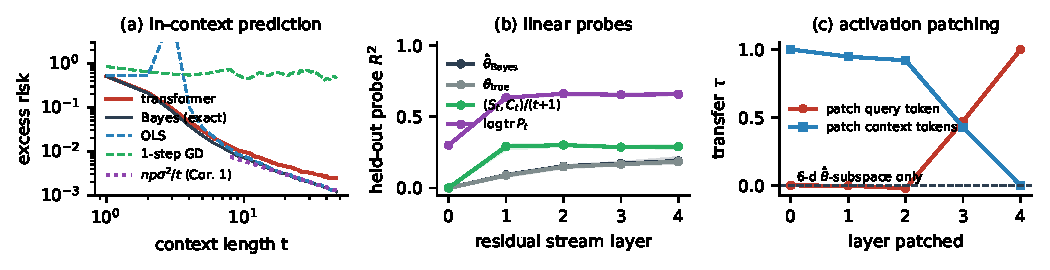
\includegraphics[width=\linewidth]{figs/fig_a.pdf}
\vspace{-6mm}
\caption{\textbf{A, pre-registered analyses} (3 seeds). (a)~Excess risk vs.\ context length. The transformer tracks the
exact Bayes predictor while data are scarce, then flattens at an approximation floor. The Bayes curve follows the
parameter-free law of Cor.~\ref{cor:law}. (b)~Held-out linear probes of the residual stream (band: range over
seeds). The estimate $\hat\theta_t$ is barely decodable; the posterior uncertainty is. (c)~Activation patching of
episode $A$ into $B$. Patching the query token transfers $A$'s behaviour only from layer~3 on. Patching the 6-d
$\hat\theta$-probe subspace transfers nothing (dashed).}
\label{fig:a}
\vspace{-3mm}
\end{figure}

\paragraph{Behaviour: Bayes-optimal while data are scarce, then an approximation floor.} The trained predictor is
much closer to the exact Bayes predictor than to OLS or to one GD step. The mean algorithmic distance to OLS exceeds
the distance to Bayes by \AdOLS\ \AdOLSci, and the distance to GD exceeds it by \AdGD\ \AdGDci\ (H1a, H1b; Holm $p\PHonea$,
$\PHoneb$). For $t\le4$ its excess risk is within a factor \Ashort\ of Bayes. After that it decays more slowly than $1/t$ and
settles about $\Afloor\times10^{-3}$ above Bayes. Meanwhile $t\,\mathcal{R}^\star_t$ reaches \AtBayes\ at $t{=}47$:
Theorem~\ref{thm:bayes} gives \AtTheory\ and Corollary~\ref{cor:law} predicts $np\sigma^2{=}0.06$. The pre-registered
tolerance H1c is \textbf{rejected}: the mean excess ratio is \Aratio\ \Aratioci, against a threshold of $1.25$. This is
the dynamical analogue of the observation that trained transformers fall short of least-squares
rates~\citep{hill2025transformers,cole2025incontext}. Longer training and larger models narrow the gap but do not
close it (\S\ref{sec:scale}).

\paragraph{The pre-registered mechanism is rejected: no estimate in the residual stream.} The best linear probe of
the residual stream for $\hat\theta_t$ reaches only $R^2{=}\ARtheta$ \ARthetaci\ (H2a, threshold $0.8$:
rejected). It beats the probe for the true $\theta$ by just \AdR\ (H2b: significant but negligible). The normalised
sufficient statistics are partly decodable ($R^2{\le}\Amom$) and peak at layers 1--2, before $\hat\theta$ peaks at
layer~4, in every seed. So H2c holds formally but is uninformative. What \emph{is} linearly decodable is the
model's uncertainty: $\log\operatorname{tr}P_t$ reaches $R^2{=}\Alogtr$. Steering along the $\hat\theta$-probe
directions does not move the prediction (slope \Aslope; H3a rejected). Swapping the 6-d probe subspace of the query
between episodes transfers $\tau{=}\Atausub$ of the behaviour, which is less than a random 6-d subspace (\Ataurand; H3b
rejected). Whole-stream patching (Fig.~\ref{fig:a}c) shows that parameter information enters the query position
only in blocks 3--4: $\tau_{\rm last}{=}\AtauLastThree$ after block~3, while patching all context positions at
layer~2 still transfers $\ge\AtauCtxTwo$.

\begin{figure}[t]
\centering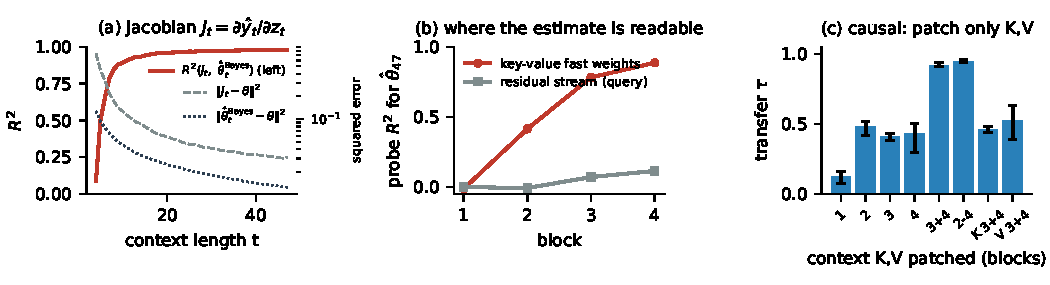
\includegraphics[width=\linewidth]{figs/fig_mech.pdf}
\vspace{-6mm}
\caption{\textbf{A, exploratory follow-up: where the estimate lives} (3 seeds). (a)~The predictor's Jacobian with
respect to its query, $J_t{=}\partial\hat y_t/\partial z_t$, matches the Bayes estimate. Its error to the truth
(dashed) tracks the Bayes estimate's error (dotted). (b)~$\hat\theta_{47}$ is linearly readable from the per-block
key--value fast weights $\widehat{\mathrm{Cov}}(v,k)$ but not from the residual stream at the same position.
(c)~Patching \emph{only} the context keys and values of blocks 3--4, leaving every activation of the query untouched,
transfers over 90\% of the other episode's behaviour. Keys or values alone transfer about half.}
\label{fig:mech}
\vspace{-3mm}
\end{figure}

\paragraph{Exploratory: the estimate lives in the keys and values, and acts through the query Jacobian.} The
following analyses were added after the pre-registered ones failed, and they are labelled as such. Remark~\ref{rem:fw}
suggests where to look.
\begin{itemize}
\item \emph{The answer is linearly represented; the parameter is not.} A linear probe recovers the Bayes
\emph{prediction} $\hat\theta_tz_t$ with $R^2{=}\AyhatLthree$ after block~3 and $\AyhatLfour$ after block~4. An MLP probe
recovers $\hat\theta_t$ itself only up to $R^2{=}\AmlpTheta$.
\item \emph{The Jacobian is the estimate.} The predictor is close to linear in its own query: counterfactual queries are explained with
$R^2{=}\AcfLin$ by its Jacobian, and their effect has slope \AcfSlope\ against the Bayes map. Its Jacobian
$J_t{=}\partial\hat y_t/\partial z_t$ matches $\hat\theta^{\rm Bayes}_t$ with $R^2{=}\AjacBayes$, more closely than it
matches the truth ($\AjacTrue$) or OLS ($\AjacOLS$) (Fig.~\ref{fig:mech}a).
\item \emph{It is stored in key--value memory.} The per-head fast weights $\widehat{\mathrm{Cov}}(v,k)$ of
block~4 predict $\hat\theta_{47}$ with $R^2{=}\AfwR$ (block 3: \AfwRthree). The residual stream at the same position
gives at most \AresidR\ (Fig.~\ref{fig:mech}b).
\item \emph{The memory is causal.} Replacing only the context keys and values of blocks 3--4 by those of another episode,
with the query's residual stream, its attention queries and all MLPs left as they were, transfers $\tau{=}\AkvThreeFour$ of that
episode's behaviour (blocks 2--4: \AkvTwoFour). Keys alone give \AkOnly\ and values alone \AvOnly
(Fig.~\ref{fig:mech}c). The carriers are 2--3 heads per block with near-uniform attention, as in Remark~\ref{rem:fw}.
\item \emph{Probe directions are not the model's directions.} Even for the well-decoded prediction, steering along the
probe direction has slope only \AsteerYhat, and swapping the probe subspace transfers only \AtauYhat. Linear decodability did not imply
causal use anywhere in this study.
\end{itemize}
In short, the transformer does implement near-Bayes system identification. It does not do so by writing $\hat\theta$
into an activation. The estimate is spread over the key--value memory of the context and is read out, applied to the query, by
attention. This is why RMA-style ``latent parameter'' probes of the residual stream~\citep{kumar2021rma,chamachot2026evaluating}
can fail even when adaptation works.

\section{Experiment B: nonlinear and contact physics in MuJoCo}\label{sec:expb}

\begin{figure}[t]
\centering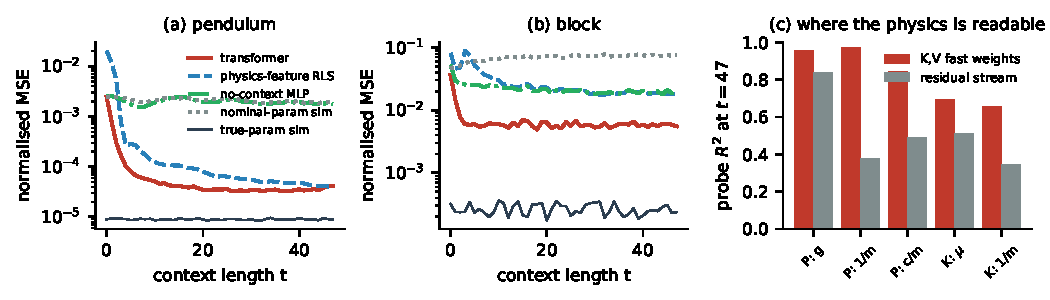
\includegraphics[width=\linewidth]{figs/fig_b.pdf}
\vspace{-6mm}
\caption{\textbf{B} (3 seeds). (a, b)~Normalised one-step error vs.\ context length. On the pendulum the transformer
beats physics-feature RLS, even though RLS has the true model class up to discretisation. On the stick--slip block it beats RLS by $3\times$. (c)~Residual-stream probes
(fixed final-position probe applied at every $t$).}
\label{fig:b}
\vspace{-3mm}
\end{figure}

\paragraph{Prediction.} Averaged over $t{=}24..47$, the normalised error on the pushed block with Coulomb friction is
\BKTF\ for the transformer and \BKRLS\ for physics-feature RLS (H4a: difference \HfourA\ \HfourAci, Holm $p\PHfoura$).
For comparison, the no-context MLP gets \BKMLP, nominal-parameter simulation \BKNom, and simulation with the true parameters
\BKOrc. On the pendulum, where feature RLS has the right model class up to discretisation, the transformer
(\BPTF) still beats it (\BPRLS). Nominal simulation (\BPNom) and the no-context MLP (\BPMLP) are $\sim$60$\times$ worse,
so the gain comes from in-context adaptation.

\paragraph{Mechanism.} The pre-registered probes again fail for the parameters that enter the dynamics
multiplicatively. Residual-stream $R^2$ at $t{=}47$ is \BprobePg\ for $g$, \BprobePinvm\ for $1/m$ and \BprobeKmu\ for
$\mu$ (H4c rejected). Steering along the $1/m$ probe moves the input sensitivity the right way in only
\BsteerP\% (pendulum) and \BsteerK\% (block) of episodes (H4d rejected). The exploratory analyses of \S\ref{sec:expa}
transfer. The model's own sensitivity $\partial\dot q_{t+1}/\partial u_t$, its functional estimate of $1/m$, correlates
with the true $1/m$ at $r{=}\BfuncP$ on the pendulum; on the block it is $r{=}\BfuncK$, because the sensitivity is zero while stuck. The
key--value fast weights decode $1/m$ with $R^2{=}\BfwPinvm$ (residual: \BresPinvm), and on the block they decode $\mu$ at \BfwKmu\ (residual
\BresKmu). \PENDING{bouncer}

\section{Experiment C: does an in-context controller explore?}\label{sec:expc}
\PENDING{resC}

\section{Scale and training length}\label{sec:scale}
\PENDING{resScale}

\section{Discussion and limitations}\label{sec:disc}
\PENDING{discussion}


\subsection*{Generative AI use}
Generative AI tools (Claude) were used for literature search and synthesis, code implementation, mathematical
derivations, and writing. The author reviewed the content, every reported number is regenerated by the scripts in the
public repository, and the author takes responsibility for the final content.

\bibliography{refs}

\appendix
\section{Deviations from the pre-registration}\label{app:dev}
(1)~We measure excess risk against the noiseless mean $\theta z_t$ instead of as $\mathrm{MSE}-n\sigma^2$. The two have the same
expectation and ours has lower variance. (2)~$\Lambda_0{=}I$ in the information measure, which the pre-registration did not fix.
(3)~Training details not fixed by the pre-registration: the constant-gain baseline uses Adam, 1000 steps and batch 1024; the no-context MLP has
2$\times$256 units and 5000 steps. (4)~The controller uses a KV-cached incremental forward to fit in 4\,GB. It is
numerically identical to the full forward. (5)~With a prior mean $B{=}0$, pre-registered CE degenerates to $u\equiv0$;
we report it as specified. (6)~On the pendulum the parameter effects are small (nominal-parameter simulation already
has 0.5\% normalised error); we kept the design unchanged.
(7)~All analyses labelled \emph{exploratory} were added after the pre-registered probes failed: the query Jacobian,
fast-weight probes, KV-only patching, answer probes, MLP probes, the bouncing-ball system, the Thompson-sampling
baseline and the scale study. (8)~\emph{Controller training.} Pure closed-loop BPTT on the cost, as pre-registered, was
unstable in pilots (Table~\ref{tab:pilots}). The final controller uses a DAgger warm start (imitating the oracle LQR
action from its own history) followed by BPTT fine-tuning on $\log(J/J_{\rm oracle})$, with 8-step truncation and
learning rate $10^{-4}$, for the pre-registered 6000 BPTT steps. (9)~Execution only: BPTT is replayed as a CUDA graph; the
constant-gain baselines are trained on the CPU. The full log is in \texttt{docs/DEVIATIONS.md}.

\section{Implementation details}\label{app:impl}
\textbf{Exact Bayes predictor (A).} Each row of $\theta$ has the Gaussian posterior of Theorem~\ref{thm:bayes}, and
the rows share their covariance. We draw 2048 joint samples, discard those with $\rho(A)\ge0.95$, and average. The
acceptance rate is \AaccZero{} at $t{=}0$ and \AaccLast{} at $t{=}47$.
\textbf{Probes.} Ridge regression on standardised residuals, with $\alpha$ chosen by 5-fold CV grouped by episode,
fitted on 2048 test episodes and scored on the other 2048. \textbf{Steering.} Let $D$ be the probe readout matrix. The
minimal-norm residual change that moves readout coordinate $k$ by $\delta$ while leaving the others unchanged is
$\delta\,(D^+)_k$. \textbf{Patching transfer} is
$\tau=\langle\hat y_{\rm patch}-\hat y_B,\hat y_{A'}-\hat y_B\rangle/\|\hat y_{A'}-\hat y_B\|^2$, where $A'$ is
episode $A$'s context followed by episode $B$'s query token. \textbf{Compute.} Everything runs on a laptop RTX~3050\,Ti
(4\,GB) with a 20-thread CPU, in about \PENDING{hours} hours end to end.

\begin{table}[h]
\centering\small
\caption{Controller-training pilots (seed 99, 1024 held-out plants). Cost is $J/J_{\rm oracle}$; ``fail'' means $J/J_{\rm oracle}{>}10$. $^\dagger$Intended lr $10^{-4}$, but a bug ran these pilots at $3{\cdot}10^{-4}$. The final runs use $10^{-4}$.}\label{tab:pilots}
\begin{tabular}{lrrrr}
\toprule
variant & step & median & mean & fail \\
\midrule
BPTT, $J/J_{\rm oracle}$, lr $3{\cdot}10^{-4}$ & 1000 & 10.49 & 298 & 51\% \\
 & 1999 & 84.89 & 1146 & 96\% \\
BPTT, $\log(J/J_{\rm oracle})$, lr $3{\cdot}10^{-4}$ & 1000 & 2.41 & 300 & 21\% \\
 & 1999 & 11.67 & 976 & 52\% \\
BPTT, $\log$, squashed inputs$^\dagger$ & 1000 & 137.67 & 76387 & 98\% \\
 & 1999 & 156.09 & 51593 & 98\% \\
same, 8-step truncated BPTT & 1000 & 4.35 & 6542 & 36\% \\
DAgger warm start (3000) + fine-tune (1500)$^\dagger$ & 0 & 2.69 & 204 & 19\% \\
 & 1000 & 2.09 & 1070 & 24\% \\
 & 1499 & 1.99 & 250 & 16\% \\
\bottomrule
\end{tabular}
\end{table}

\PENDING{appextra}


\end{document}
